%!TEX encoding = UTF-8 Unicode
% $Id: 7-macros.tex 17 2014-03-09 13:05:41Z binghe $

\chapter{宏}
\label{chap:macros}
\index{macros 宏}
\index{macros 宏|seealso {backquote, read-macro, symbol-macros}}

Lisp 中,宏的特性让你能用变换的方式定义操作符。宏定义\index{macros 宏!defining}在本质上,是能
生成~Lisp 代码的函数\pozhehao{}一个能写程序的程序。这一小小开端引发了巨大 
的可能性,同时也伴随着难以预料的风险。
第~\ref{chap:macros}--\ref{chap:other_macro_pitfalls} 章将带你走入宏的
世界。本章会解释宏如何工作,介绍编写和调试它们的技术,然后分析一些宏风
格中存在的问题。

\section{宏是如何工作的}
\label{sec:how_macros_work}

由于我们可以调用宏并得到它的返回值,因此宏往往被人们和函数联系在一起。宏定义有时和
函数定义相似,而且不严谨地说,被人们称为~``内置函数'' 的~\texttt{do} 其实就是一
个宏。但如果把两者过于混为一谈,就会造成很多困惑。宏和常规函数的工作方式
截然不同,并且只有知道宏为何不同,以及怎样不同才是用好它们的关键。一个函数只产
生结果,而宏却产生\emph{表达式}\pozhehao{}当它被求值时,才会产生结果。

要入门,最好的办法就是直接看个例子。假设我们想要写一个
宏~\texttt{nil!},它把实参设置为~\verb|nil|。让~\verb|(nil! x)|
和~\texttt{(setq x nil)} 的效果一样。我们完成这个功能的方法
是:把~\texttt{nil!} 定义成宏,让它来把前一种形式的实例变成后一
种形式的实例。
\begin{lstlisting}
> (defmacro nil! (var)
    (list 'setq var nil))
NIL!
\end{lstlisting}
\index{defmacro@\texttt{defmacro}}
用汉语转述的话,这个定义相当于告诉~Lisp: ``无论何时,只要看到形
如~\texttt{(nil! $var$)} 的表达式,请在求值之前先把它转化
成~\texttt{(setq $var$ nil)} 的形式。''

宏产生的表达式将在调用宏的位置求值。宏调用是一个列表,列表的第一个元素是
宏的名称。当我们把宏调用~\texttt{(nil! x)} 输入到~toplevel 的时候发生了
什么? Lisp 首先会发觉~\texttt{nil!} 是个宏的名字,然后
\begin{enumerate}
 \item 按照上述定义的要求构造表达式,接着
 \item 在调用宏的地方求值该表达式。
\end{enumerate}

构造新表达式的那一步被称为\emph{宏展
  开~(macroexpansion)}\index{macros 宏!expansion of}。Lisp 查
找~\texttt{nil!} 的定义,其定义展示了如何为宏调用构建一个即将取代它的表
达式。和函数一样,\texttt{nil!} 的定义也应用到了宏调用传给它
的\emph{表达式}参数上。它返回一个三元素列表,这三个元素分别是:
\texttt{setq}、作为参数传递给宏的那个表达式,以及~\texttt{nil}。在本例
中,\texttt{nil!} 的参数是~\texttt{x},宏展开式是~\texttt{(setq x
  nil)}。

宏展开之后是第二步:\emph{求值~(evaluation)}。Lisp 求值宏展开
式~\texttt{(setq x nil)} 时就好像是你原本就写在那儿的一样。求值并不总是
立即发生在展开之后,不过在~toplevel 下的确是这样的。一个发生在函数定
义里的宏调用将在函数编译时展开\index{macros 宏!compiled}, 但展开式\pozhehao{}或者说它产生的对象代
码\pozhehao{}要等到函数被调用时才会求值。

如果把宏的展开和求值分清楚,你遇到的和宏有关的困难,或许有很多就能避免。
当编写宏的时候,要清楚哪些操作是在宏展开期进行的\index{macros 宏!expansion of!time of},而哪些操作是在求值期
进行的,通常,这两步操作的对象截然不同。宏展开步骤处理的是表达式,而求
值步骤处理的则是它们的值。

有些宏的展开过程比~\texttt{nil!} 的情况更复杂。\texttt{nil!} 的展开
式只是调用了一下内置的~special form,但往往一个宏的展开式可能会是另一个宏
调用,就好像是一层套一层的俄罗斯套娃。在这种情况下,宏展开就会继续抽丝剥
茧直到获得一个没有宏的表达式。这一步骤中可以经过任意多次的展开操作,一
直到最终停下来。

尽管有许多语言也提供了某种形式的宏,但~Lisp 宏却格外强大。在编译~Lisp
文件时,解析器先读取源代码,然后将其输出送给编译器。这里有个天才的手
笔:解析器的输出由\emph{~Lisp 对象的列表}组成。通过使用宏,我们可以操
作这种处于解析器和编译器之间的中间状态的程序。如果必要的话,这些操作可
以无所不包。一个生成展开式的宏拥有~Lisp 的全部威力,可任其驱驰。事实
上,宏是货真价实的~Lisp 函数\pozhehao{}那种能返回表达式的函数。虽
然~\texttt{nil!} 的定义中只是调用了一下~\texttt{list},但其他宏里可能会
驱动整个子程序来生成其展开式。

有能力改变编译器所看到的东西,差不多等同于能够对代码进行重写。所以我们就可以为语言
增加任何构造,只要用变换的方法把它定义成已有的构造。

\section{\bq{}~(backquote)}
\label{sec:backquote}

\bq{}~(backquote)\index{backquote@backquote (\texttt{`}) \bq{}} 是引用~(quote)\index{quote@\texttt{quote}} 的特别
版本,它可以用来创建~Lisp 表达式的模板。\bq{}最常见的用途之一是用在宏定义里。

\bq{}字符``\texttt{`}''得名的原因是:它和通常的引号``\texttt{'}''相似,只
不过方向相反。当单独把\bq{}作为表达式前缀的时候,它的行为和引号一样:
\begin{equation*}
  \mbox{\texttt{`(a b c)} 等价于~\texttt{'(a b c)}.}
\end{equation*}

%% xxx
只有在\bq{}和\comma{}``\texttt{,}''\index{,@\texttt{,}},以及~comma-at
``\texttt{,@}''一同出现时才变得有用。如果说\bq{}创建了一个模
板,那么\comma{}就在\bq{}中创建了一个~slot。一个\bq{}列表等价于将其元素
引用起来,调用一次~\texttt{list}。也就是,
\begin{equation*}
  \mbox{\texttt{`(a b c)} 等价于~\texttt{(list 'a 'b 'c)}.}
\end{equation*}
在\bq{}的作用域里,\comma{}要求~Lisp:“把引用关掉”。当\comma{}出现在列表
元素前面时,它的效果就相当于取消引用,让~Lisp 把那个元素按原样放在那里。所以
\begin{equation*}
  \mbox{\texttt{`(a ,b c ,d)} 等价于~\texttt{(list 'a b 'c d)}.}
\end{equation*}
插入到结果列表里的不再是符号~\texttt{b},取而代之的是它的值。无论\comma{}在嵌套列表里
的层次有多深,它都仍然有效,
\begin{lstlisting}
> (setq a 1 b 2 c 3)
3
> `(a ,b c)
(A 2 C)
> `(a (,b c))
(A (2 C))
\end{lstlisting}
而且它们也可以出现在引用的列表里,或者引用的子列表里:
\begin{lstlisting}
> `(a b ,c (',(+ a b c)) (+ a b) 'c '((,a 'b)))
(A B 3 ('6) (+ A B) 'C '((1 'B)))
\end{lstlisting}

一个\comma{}能抵消一个\bq{}的效果,所以\comma{}在数量上必须和\bq{}匹配。如果某个
操作符出现在\comma{}的外层,或者出现在包含\comma{}的那个表达式的外层,那么我们说
该操作符\emph{包围}了这个\comma{}。例如在~\texttt{`(,a ,(b `,c))} 中,
最后一个\comma{}就被
前一个\comma{}和两个反引号所包围。通行的规则是:一个被~$n$ 个\comma{}包围的\comma{}必须被至少
~$n+1$ 个反引号所包围。很明显,由此可知:\comma{}不能出现在\bq{}的表达式的外面
。只要遵守上述规则,就可以嵌套使用\bq{}和\comma{}。下面的任何一个表达式如果输入到
~toplevel 下都将造成错误:
\begin{center}
  \verb|,x|\qquad\verb|`(a ,,b c)|\qquad\verb|`(a ,(b ,c) d)|\qquad\verb|`(,,`a)|
\end{center}
嵌套的\bq{}只有在宏定义的宏里才可能会用到。
第~\ref{chap:macro-defining_macros} 章将讨论这两个主题。

\bq{}通常被用来创建列表。\footnote{\bq{}也可以用于创建向量~(vector)\index{vectors 向量!creating with backquote 用\bq{}来创建},不过这个
用法很少在宏定义里出现。}任何用\bq{}生成的列表也都可以用~\texttt{list} 和
普通的引用来实现。使用\bq{}的好处只是在于它改进了表达式的可读性,因为反
引用的表达式和它将生成的表达式很相似。在前一章里我们把~\texttt{nil!} 定义成:
\begin{lstlisting}
(defmacro nil! (var)
  (list 'setq var nil))
\end{lstlisting}
借助\bq{},这个宏可以定义成:
\begin{lstlisting}
(defmacro nil! (var)
  `(setq ,var nil))
\end{lstlisting}
在本例中,是否使用\bq{}的差别还不算太大。不过,随着宏定义长度的增加,\bq{}也会变得愈加重要。
图~\ref{fig:a_macro_defined_with_and_without_backquote} 包含了两个
~\texttt{nif}\label{mac:nif}
可能的定义,这个宏实现了三路数值条件选择。
\footnote{这个宏的定义稍微有些不自然,这是为了避免使用~gensym。
在第~\pageref{fig:macros_for_conditional_evaluation} 页上有一个更好的定义。}

\begin{figure}
使用\bq{}:
\begin{lstlisting}
(defmacro nif (expr pos zero neg)
  `(case (truncate (signum ,expr))
     (1 ,pos)
     (0 ,zero)
     (-1 ,neg)))
\end{lstlisting}
不使用\bq{}:
\begin{lstlisting}
(defmacro nif (expr pos zero neg)
  (list 'case
     (list 'truncate (list 'signum expr))
     (list 1 pos)
     (list 0 zero)
     (list -1 neg)))
\end{lstlisting}
\index{nif@\texttt{nif}}
\index{signum@\texttt{signum}}
\caption{\label{fig:a_macro_defined_with_and_without_backquote}一个使用和不使
用\bq{}的宏定义。}
\end{figure}

首先,第一个参数会被求值成数字。然后会根据这个数字的正负、是否为零,来决定第二、第
三和第四个参数中哪一个将被求值:

\begin{lstlisting}
> (mapcar #'(lambda (x)
              (nif x 'p 'z 'n))
          '(0 2.5 -8))
(Z P N)
\end{lstlisting}

图~\ref{fig:a_macro_defined_with_and_without_backquote} 中的两个定义分
别定义了同一个宏,但是前者使用的是\bq{},而后者则通过显式调
用~\texttt{list} 来构造它的展开式。以~\texttt{(nif x 'p 'z
  'n)} 为例,从第一个定义中很容易就能看出来,这个表达式会展开成
\begin{lstlisting}
(case (truncate (signum x))
  (1 'p)
  (0 'z)
  (-1 'n))
\end{lstlisting}
因为这个宏定义体的模样就和它生成的宏展开式差不多。要想理解不使用\bq{}的第
二个版本,你将不得不在脑海中重演一遍展开式的构造过程。

comma-at,即``\texttt{,@}\index{,"@@\texttt{,"@}}'',是\comma{}的变
形,其行为和\comma{}相似,但有一点不同: comma-at 不像\comma{}那样仅仅把
表达式的值插入到所在的位置,而是把表达式\emph{拼接}\index{splicing 拼接}进去。拼接这个操作
可以这样理解:在插入的同时,剥去被插入对象最外层的括号:
\begin{lstlisting}
> (setq b '(1 2 3))
(1 2 3)
> `(a ,b c)
(A (1 2 3) C)
> `(a ,@b c)
(A 1 2 3 C)
\end{lstlisting}

\comma{}导致列表~\texttt{(1 2 3)} 被插入到~\texttt{b} 所在的位置,而~comma-at~把列表中的元素
插入到那里。对于~comma-at~的使用,还另有限制:
\begin{enumerate}
\item 为了确保其参数可以被拼接,comma-at~必须出现在序列~(sequence)
\footnote{译者注:序列~(sequence) 是~Common Lisp 标准定义的数据类型,它的两个子
类型分别是列表~(list) 和向量~(vector)。}中。形如~\texttt{`,@b} 的说法是错误的,因为无处
可供~\texttt{b} 的值进行拼接。
\item 要进行拼接的对象必须是个列表,除非它出现在列表最后。
表达式~\texttt{`(a ,@1)} 将被求值成~\texttt{(a . 1)},但如果尝试将
原子\footnote{译者注:原子~(atom) 也是~Common Lisp 标准定义的数据类型,所
有不是列表的~Lisp 对象都是原子,包括向量~(vector) 在内。}~(atom) 拼接到列表
的中间位置,例如~\texttt{`(a ,@1 b)},将导致一个错误。
\end{enumerate}

comma-at~一般用在接受不确定数量参数的宏里,以及将这些参数传给同样接受不确定
数量参数的函数和宏里。这一情况通常广泛用于实现隐式的块~(block)。Common Lisp
提供几种将代码分组到块的操作符,包括~\texttt{block}、\texttt{tagbody}, 以及
~\texttt{progn}。这些操作符很少直接出现在源代码里;它们一般不显山露水\pozhehao{}
而是藏身在宏的背后。

隐式块出现在任何一个带有表达式\emph{体}\index{body (of expressions) 体~(表达式)}的内置宏里。例如~\texttt{let} 和
~\texttt{cond} 里都有隐式的~\texttt{progn} 存在。做这种事情的内建宏里,最简单的
一个可能要算~\texttt{when} 了:
\begin{lstlisting}
(when (eligible obj)
  (do-this)
  (do-that)
  obj)
\end{lstlisting}
如果~\texttt{(eligible obj)} 返回真,那么其余的表达式将会被求值,并且整个
~\texttt{when} 表达式会返回其中最后一个表达式的值。下面是一个使用~comma-at 的示例,
它是~\texttt{when} 的一种可能的实现:
\begin{lstlisting}
(defmacro our-when (test &body body)
  `(if ,test
       (progn
         ,@body)))
\end{lstlisting}
这一定义使用了一个~\texttt{\&body}\index{body@\texttt{\&body}} 参数~(它和~\texttt{\&rest}\index{rest@\texttt{\&rest} parameters} 功能相同,只有美观
输出的时候不太一样) 来接受可变数量的参数,然后一个~comma-at~将它们拼接到一个
~\texttt{progn} 表达式里。在上述调用的宏展开式里,宏调用体里面的三个表达式将
出现在单个~\texttt{progn} 中:
\begin{lstlisting}
(if (eligible obj)
    (progn (do-this)
           (do-that)
           obj))
\end{lstlisting}

多数需要迭代处理其参数的宏都采用类似方式拼接它们。

comma-at~的效果也可以不用\bq{}实现。例如,表达式~\verb|`(a ,@b c)| 就和
~\verb|(cons 'a (append b (list 'c)))| 等价。之所以用上~comma-at,
只是为了改进这种由表达式生成的表达式的可读性。

宏定义~(通常) 生成列表。尽管宏展开式可以用函数~\verb|list| 来生成,但\bq{}的
列表模板可以令这一任务更为简单。用~\verb|defmacro| 和\bq{}定义的宏,在形式
上和用~\verb|defun| 定义的函数非常相似。只要不被这种相似性误导,\bq{}
就能让宏定义既容易书写也方便阅读。

由于\bq{}经常出现在宏定义里,以致于人们有时误以为\bq{}是~\verb|defmacro| 的一部分。
关于\bq{}的最后一件要记住的事情,是它有自己存在的意义,这跟它在宏定义中的角色无关。
你可以在任何需要构造序列的场合使用\bq{}:
\begin{lstlisting}
(defun greet (name)
  `(hello ,name))
\end{lstlisting}

\section{定义简单的宏}
\label{sec:defining_simple_macros}
\index{macros 宏!simple}

在编程领域,最快的学习方式通常是尽快地开始实践。完全理论上的理解可以稍后再说。
因此本章介绍一种可以立即开始编写宏的方法。虽然该方法的适用范围很窄,但在这个
范围内却可以高度机械化地实现。(如果你以前写过宏,可以跳过本节。)

下面举个例子,让我们考虑一下如何写出~Common Lisp 内置函
数~\verb|member|\index{member@\texttt{member}} 的
变形。\verb|member| 缺省用~\verb|eql| 来判断等价与否。如果你想要
用~\verb|eq| 来判断是否等价,你就必须显式写成这样:
\begin{lstlisting}
(member x choices :test #'eq)
\end{lstlisting}

如果常常这样做,那我们可能会想要写一个~\verb|member| 的变形,让它总是
使用~\verb|eq|。有些早期的~Lisp 方言就有这样的一个函数,叫
做~\verb|memq|\index{memq@\texttt{memq}}:
\begin{lstlisting}
(memq x choices)
\end{lstlisting}
通常应该将~\texttt{memq} 定义为内联~(inline) 函数,但为了举例子,我们会
让它以宏的面目出现。

\begin{figure}
  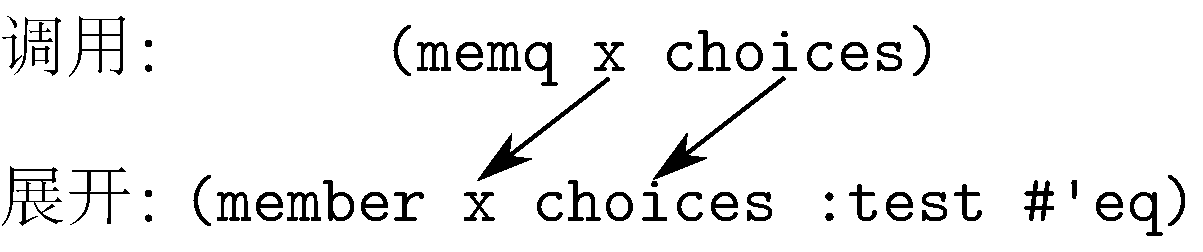
\includegraphics[width=.46\textwidth]{memq.pdf}
  \caption{\label{fig:diagram_used_in_writing_memq}用于写~\texttt{memq} 的图示}
\end{figure}

方法如下:从你想要定义的这个宏的一次典型调用开始。先把它写在纸上,然后下面写上
它应该展开成的表达式。图~\ref{fig:diagram_used_in_writing_memq} 给出了两个这样
的表达式。通过宏调用,构造出你这个宏的参数列表,同时给每个参数命名。
这个例子中有两个实参,所以我们将会有两个形参,把它们叫做~\verb|obj|
和~\verb|lst|:
\begin{lstlisting}
(defmacro memq (obj lst)
\end{lstlisting}
现在回到之前写下的两个表达式。对于宏调用中的每个参数,画一条线把它和它
在展开式里出现的位置连起来。图~\ref{fig:diagram_used_in_writing_memq} 中有
两条并行线。为了写出宏的实体,把你的注意力转移到展开式。让主体以\bq{}开头。
现在,开始逐个表达式地阅读展开式。每当发现一个括号,如果它不是宏调用中实参
的一部分,就把它放在宏定义里。所以紧接着\bq{}会有一个左括号。对于展开式里的每个
表达式
\begin{enumerate}
\item 如果没有线将它和宏调用相连,那么就把表达式本身写下来。
\item 如果存在一条跟宏调用中某个参数的连接,就把出现在宏参数列表的对应位置的那个
  符号写下来,前置一个\comma{}。
\end{enumerate}
由于第一个元素~\verb|member| 上没有连接,所以我们照原样使用~\verb|member|:
\begin{lstlisting}
(defmacro memq (obj lst)
  `(member
\end{lstlisting}
不过,\verb|x| 上有一条线指向源表达式中的第一个实参,所以我们在宏的主体
中使用第一个参数,带一个\comma{}:
\begin{lstlisting}
(defmacro memq (obj lst)
  `(member ,obj
\end{lstlisting}
以这种方式继续进行,最后完成的宏定义是:
\begin{lstlisting}
(defmacro memq (obj lst)
  `(member ,obj ,lst :test #'eq))
\end{lstlisting}

\begin{figure}
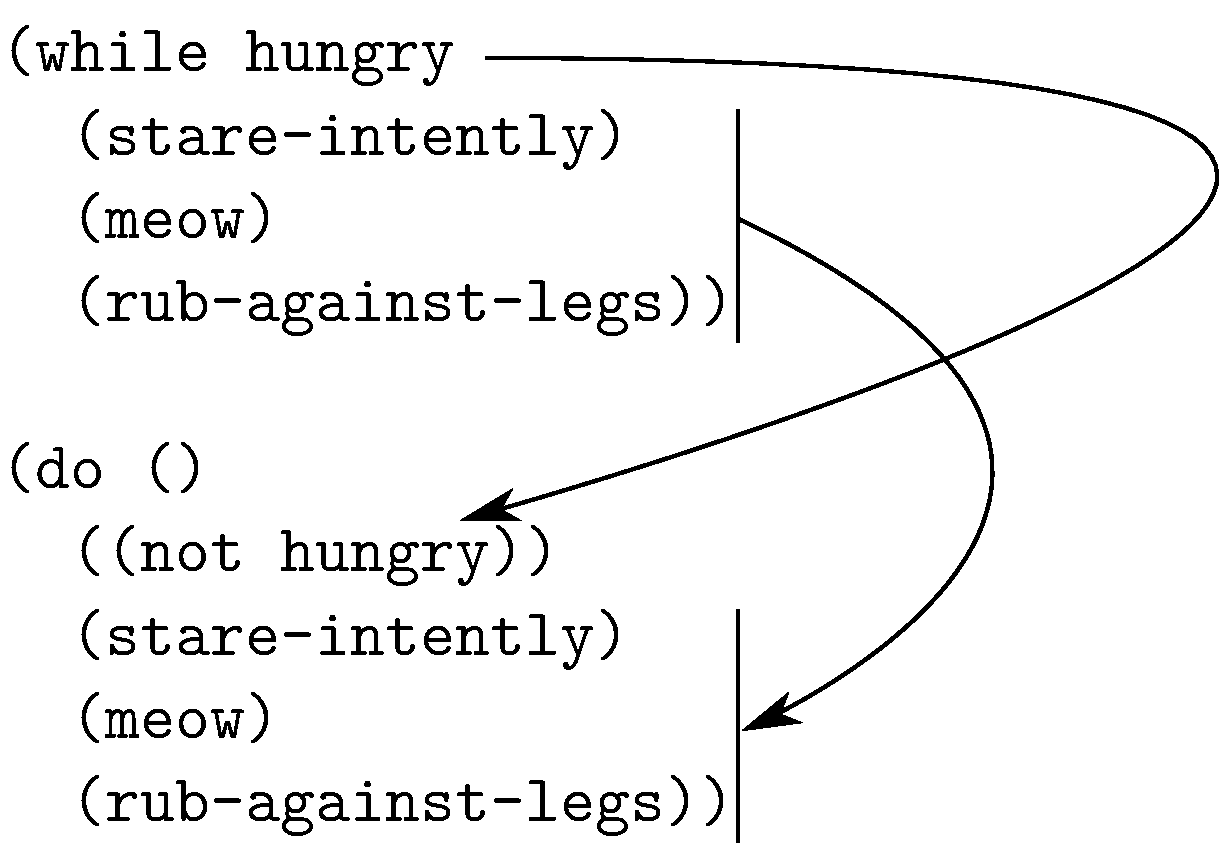
\includegraphics[width=.46\textwidth]{while.pdf}
\caption{\label{fig:diagram_used_in_writing_while}用于写~\texttt{while} 的图示}
\end{figure}

到目前为止,我们写出的宏,其参数个数只能是固定的。现在假设我们打算写一
个~\verb|while| 宏,它接受一个条件表达式和一个代码体,然后循环执行代
码直到条件表达式返回真。图~\ref{fig:diagram_used_in_writing_while} 含有
一个描述猫的行为的~\verb|while| 循环示例。

要写出这样的宏,我们需要对我们的技术稍加修改。和前面一样,先写一个宏
调用作为毛坯。然后,以它为基础,构造宏的形参列表,其中,在想要接受任意多
个参数的地方,以一个~\verb|&rest| 或~\verb|&body| 形参作结:
\begin{lstlisting}
(defmacro while (test &body body)
\end{lstlisting}
现在,在宏调用的下面写出目标展开式,并且和之前一样,画线把宏调用的形参和
它们在展开式中的位置连起来。然而,当你碰到一个系列形参,而且它们会
被~\verb|&rest| 或~\verb|&body| 实参吸收时,就要把它们当成一组
处理,并只用一条线来连接整个参数序列。
图~\ref{fig:diagram_used_in_writing_while} 给出了最后的图示。

为了写出宏定义的主体,按之前的步骤处理表达式。在前面给出的两条规则之外,
我们还要加上一条:
\begin{enumerate}
\setcounter{enumi}{2}
\item 如果在一系列展开式中的表达式和宏调用里的一系列形参之间存在联系,那么
  就把对应的~\verb|&rest| 或~\verb|&body| 实参记下来,在前面加上~comma-at。
\end{enumerate}
于是宏定义的结果将是:\label{macro:while}
\begin{lstlisting}
(defmacro while (test &body body)
  `(do ()
       ((not ,test))
     ,@body))
\end{lstlisting}
要想构造带有表达式\emph{体}\index{body (of expressions) 体~(表达式)}的宏,就必须有参数充当打包装箱的角色。这里宏调用中的
多个参数被串起来放到~\verb|body| 里,然后在~\verb|body| 被拼接进展开式时,再把它
拆散开。

用本章所述的这个方法,我们能写出最简单的宏\pozhehao{}这种宏只能在参数位置上做
文章。但是宏可以比这做的多得多。第~\ref{sec:macros_as_programs} 章将会举
一个例子,这个例子无法用简单的\bq{}列表表达,并且为了生成展开式,例子中的
宏成为了真正意义上的程序。

\section{测试宏展开}
\label{sec:testing333_macroexpansion}

宏写好了,那我们怎么测试它\index{macros 宏!testing 测
  试}呢?像~\verb|memq| 这样的宏,它的结构较简单,只消看看它的代码就
能弄清其行为方式。而当编写结构更复杂的宏时,我们必须有办法检查它们展开
之后正确与否。

\begin{figure}
\begin{lstlisting}
> (defmacro while (test &body body)
    `(do ()
         ((not ,test))
       ,@body))
WHILE

> (pprint (macroexpand '(while (able) (laugh))))

(BLOCK NIL
  (LET NIL
    (TAGBODY
      #:G61
      (IF (NOT (ABLE)) (RETURN NIL))
      (LAUGH)
      (GO #:G61))))
T
> (pprint (macroexpand-1 '(while (able) (laugh))))

(DO NIL
    ((NOT (ABLE)))
  (LAUGH))
T
\end{lstlisting}
\caption{\label{fig:a_macro_and_two_depths_of_expansion}一个宏和它的两级展开}
\end{figure}

图~\ref{fig:a_macro_and_two_depths_of_expansion} 给出了一个宏定义和用
来查看其展开式的两个方法。内置函
数~\verb|macroexpand|\index{macroexpand@\texttt{macroexpand}} 的参数
是个表达式,它返回这个表达式的宏展开式。把一个宏调用传
给~\verb|macroexpand|,就能看到宏调用在求值之前最终展开的样
子,但是当你测试宏的时候,并不是总想看到彻底展开后的展开式。如果有宏
依赖于其他宏,被依赖的宏也会一并展开,所以完全展开后的宏有时是不利于
阅读的。

从图~\ref{fig:a_macro_and_two_depths_of_expansion} 给出的第一个表
达式,很难看出~\texttt{while} 是否如愿展开,因为不仅内置的
宏~\texttt{do} 被展开了,而且它里面的~\texttt{prog} 宏也展开了。我们需
要一种方法,通过它能看到只展开过一层宏的展开结果。这就是内置函
数~\texttt{macroexpand-1}\index{macroexpand-1@\texttt{macroexpand-1}}
的目的,正如第二个例子所示。就算展开后,得到的结果仍然是宏调
用,\texttt{macroexpand-1} 也只做一次宏展开就停手。

\begin{figure}
\begin{lstlisting}
(defmacro mac (expr)
  `(pprint (macroexpand-1 ',expr)))
\end{lstlisting}
\caption{\label{fig:a_macro_for_testing_macroexpansion}一个用于测试宏展开的宏}
\index{mac@\texttt{mac}}
\end{figure}

如果每次查看宏调用的展开式都得输入如下的表达式,这会让人很头痛:
\begin{lstlisting}
(pprint (macroexpand-1 '(or x y)))
\end{lstlisting}
图~\ref{fig:a_macro_for_testing_macroexpansion} 定义了一个新的宏,它让我们有一个简单的替代方法:
\begin{lstlisting}
(mac (or x y))
\end{lstlisting}

调试函数的典型方法是调用它们,同样的道理,对于宏来说就是展开它们。不过由于宏调用
涉及了两次计算,所以它也就有两处可能会出问题。如果一个宏行为不正常,大多数时候你
只要检查它的展开式,就能找出有错的地方\index{macros 宏!expansion of!testing}。不过也有一些时候,展开式看起来是对的,
所以你想对它进行求值以便找出问题所在。如果展开式里含有自由变量,你可能需要先设
置一些变量。在某些系统里,你可以复制展开式,把它粘贴到~toplevel 环境里,或者
选择它然后在菜单里选~\texttt{eval}\index{eval@\texttt{eval}!on macroexpansions}。在最坏的情况下你也可以把
~\texttt{macroexpand-1} 返回的列表设置在一个变量里,然后对它调用
~\texttt{eval}:
\begin{lstlisting}
> (setq exp (macroexpand-1 '(memq 'a '(a b c))))
(MEMBER (QUOTE A) (QUOTE (A B C)) :TEST (FUNCTION EQ))
> (eval exp)
(A B C)
\end{lstlisting}

最后,宏展开不只是调试的辅助手段,它也是一种学习如何编写宏的方式。Common Lisp
带有超过一百个内置宏,其中一些还颇为复杂。通过查看这些宏的展开过程你经常能
了解它们是怎样写出来的。

\section{参数列表的解构}
\label{sec:destructuring_in_parameter_lists}

解构~(destructuring) 是用在处理函数调用中的一种赋值操作\footnote{
解构通常用在创建变量绑定,而非~\texttt{do} 那样的操作符里。尽管如此,概念上
来讲解构也是一种赋值的方式,如果你把列表解构到已有的变量而非新变量上是完全
可行的。就是说,没有什么可以阻止你用解构的方法来做类似~\texttt{setq} 这样的
事情。}的推广形式。如果你定义的函数带有多个形参
\begin{lstlisting}
(defun foo (x y z)
  (+ x y z))
\end{lstlisting}
当调用该函数时
\begin{lstlisting}
(foo 1 2 3)
\end{lstlisting}
函数调用中实参会按照参数位置的对应关系,赋值给函数的形参:\texttt{1} 赋给 \texttt{x},\texttt{2} 赋给 \texttt{y}
,\texttt{3} 赋给 \texttt{z}。和本例中扁平列表 \texttt{(x y z)} 的情形类似,\emph{解构~(destructuring)} 同样也指定了按位置赋值的方式,不过它能按照任意一种列表结构来进行赋值。

Common Lisp 的~\texttt{destructuring-bind}\index{Common Lisp!differences between versions!destructuring-bind@\texttt{destructuring-bind}} 宏~(\textsc{cltl}2 新增) 接受一个
匹配模式,一个求值到列表的实参,以及一个表达式体,然后在求值表达式时将模式中的参数
绑定到列表的对应元素上:
\begin{lstlisting}
> (destructuring-bind (x (y) . z) '(a (b) c d)
    (list x y z))
(A B (C D))
\end{lstlisting}
这一新操作符和其它类似的操作符构成了第~\ref{chap:destructuring} 章的主题。

在宏参数列表\index{macros 宏!parameter lists}里进行解构也是可能的\index{destructuring!in macros}。Common Lisp 的~\texttt{defmacro} 宏允许任意列表
结构作为参数列表。当宏调用被展开时,宏调用中的各部分将会以类似
~\texttt{destructuring-bind} 的方式被赋值到宏的参数上面。内置的~\texttt{dolist}\index{dolist@\texttt{dolist}}
宏就利用了这种参数列表的解构技术。在一个像这样的调用里:
\begin{lstlisting}
(dolist (x '(a b c))
  (print x))
\end{lstlisting}
展开函数必须把~\verb|x| 和~\verb|'(a b c)| 从作为第一个参数给出的列表里抽取出来。
这个任务可以通过给~\texttt{dolist} 适当的参数列表隐式地完成:
\footnote{该版本用一种奇怪的方式来写以避免使用~\texttt{gensym},这个操作符以后
会详细介绍。}
\begin{lstlisting}
(defmacro our-dolist ((var list &optional result) &body body)
  `(progn
     (mapc #'(lambda (,var) ,@body)
           ,list)
     (let ((,var nil))
       ,result)))
\end{lstlisting}
% xxx
在~Common Lisp 中,类似~\texttt{dolist} 这样的宏通常把参数包在一个列表里面,而后者不属于
宏体。由于~\texttt{dolist} 接受一个可选的~\texttt{result} 参数,所以它无论
如何都必须把它参数的第一部分塞进一个单独的列表。但就算这个多余的列表结构是画蛇添足,
它也可以让~\texttt{dolist} 调用更易于阅读。假设我们想要定义一个宏
~\texttt{when-bind}\label{mac:when_bind},它的功能和~\texttt{when} 差不多,
除此之外它还能绑定一些变量到测试表达式返回的值上。这个宏最好的实现办法可能会用到一个嵌套的参数表:
\begin{lstlisting}
(defmacro when-bind ((var expr) &body body)
  `(let ((,var ,expr))
     (when ,var
       ,@body)))
\end{lstlisting}
然后这样调用:
\begin{lstlisting}
(when-bind (input (get-user-input))
  (process input))
\end{lstlisting}
而不是原本这样调用:
\begin{lstlisting}
(let ((input (get-user-input)))
  (when input
    (process input)))
\end{lstlisting}
审慎地使用它,参数列表解构技术可以带来更加清晰的代码。最起码,它可以用在诸如
~\texttt{when-bind} 和~\texttt{dolist} 这样的宏里,它们接受两个或更多的实参,
和一个表达式体。

\section{宏的工作模式}
\label{sec:a_model_of_macros}

关于``宏究竟做了什么''的形式化描述将是既拖沓冗长,又让人不得要领的。就算有经验的
程序员也记不住这样让人头晕的描述。想象一
下~\texttt{defmacro}\index{defmacro@\texttt{defmacro}} 是怎样定义的,通
过这种方式来记忆它的行为会更容易些。

\begin{figure}
\begin{lstlisting}
(defmacro our-expander (name) `(get ,name 'expander))

(defmacro our-defmacro (name parms &body body)
  (let ((g (gensym)))
    `(progn
       (setf (our-expander ',name)
             #'(lambda (,g)
                 (block ,name
                   (destructuring-bind ,parms (cdr ,g)
                     ,@body))))
       ',name)))

(defun our-macroexpand-1 (expr)
  (if (and (consp expr) (our-expander (car expr)))
      (funcall (our-expander (car expr)) expr)
      expr))
\end{lstlisting}
\caption{\label{fig:a_sketch_of_defmacro}一个~\texttt{defmacro} 的草稿}
\end{figure}

在~Lisp 里用这种方法解释概念已由来已久。早在~1962 年首次出版
的~\emph{Lisp 1.5 Programmer's Manual}\index{Lisp!1.5}\note{95},
就在书中给出了一个用~Lisp 写的~\texttt{eval} 函数的定义作为参考。
由于~\texttt{defmacro} 自身也是宏,所以我们可以依法炮制,如
图~\ref{fig:a_sketch_of_defmacro} 所示。这个定义里使用了几种我们尚未提
及的技术,所以某些读者可能需要稍后再回过头来读懂它。

图~\ref{fig:a_sketch_of_defmacro} 中的定义相当准确地再现了宏的行为,但
就像任何草稿一样,它远非十全十美。它不能正确地处
理~\texttt{\&whole}\index{whole@\texttt{\&whole}} 关键字。而且,真正
的~\texttt{defmacro} 为它第一个参数的~\texttt{macro-function} 保存的是
一个有\emph{两个}参数的函数,两个参数分别为:宏\index{macros 宏!environment argument to}调用本身,和其发生时的
词法环境\index{environment!argument}。还好,只有最刁钻的宏才会用到这些
特性。就算你以为宏就是像图~\ref{fig:a_sketch_of_defmacro} 那样实现
的,在实际使用宏的时候,也基本上不会出错。例如,在这个实现下,本书定义
的每一个宏都能正常运行。

图~\ref{fig:a_sketch_of_defmacro} 的定义里产生的展开函数是个被井号引用过的
~\lexpr。那将使它成为一个闭包:宏定义中的任何自由符号应该指向~\texttt{defmacro}
发生时所在环境\index{macros 宏!environment of expander}里的变量。所以下列代码是可行的:
\begin{lstlisting}
(let ((op 'setq))
  (defmacro our-setq (var val)
    (list op var val)))
\end{lstlisting}
上述代码对~\textsc{cltl}2 来说没有问题。但
在~\textsc{cltl}1 里,宏展开器\index{environment!of macro expanders 宏
  展开器}是在空词法环境\index{environment!null 空}里定义的\footnote{关
  于这一区别实际有影响的例子,请参见
  第~\pageref{notes:difference-null-environment} 页的注释。},所以在一
些老的~Common Lisp 实现里,这个~\texttt{our-setq} 的定义将不会正常工作。

\section{作为程序的宏}
\label{sec:macros_as_programs}
\index{macros 宏!as programs 作为程序的}

宏定义并不一定非得是个\bq{}列表。宏的本质是函数,它把一个表达式转换成另一个表达式。这
个函数可以调用 \verb|list| 来生成结果,但是同样也可以调用一整个长达数百行代码
的子程序达到这个目的。

第 \ref{sec:defining_simple_macros} 节给出了一个编写宏的简易方案。借助这一技术,
我们可以写出这样的宏,让它的展开式包含的子表达式和宏调用中的相同。不幸的是,只有最简单
的宏才能满足这一条件。现在举个复杂一些的例子,让我们来看看内置的宏 \verb|do|。
要把 \verb|do| 实现成那种只是把参数重新排列一下的宏是不可能的。在展开过程中,必须构造
出一些在宏调用中没有出现过的复杂\index{macros 宏!complex 复杂}表达式。

关于编写宏,有个更通用的方法:先想想你想要使用的是哪种表达式,再设想一下
它应该展开成的模样,最后写出能把前者变换成后者的\emph{程序}。可以试着手工展开一个
例子,分析在表达式从一种形式变换到另一种形式的过程中,究竟发生了什么。从实例出发,你就可以大致明白在你将要写的宏里将需要做些什么工作。

\begin{figure}
\begin{lstlisting}
(do ((w 3)
     (x 1 (1+ x))
     (y 2 (1+ y))
     (z))
    ((> x 10) (princ z) y)
  (princ x)
  (princ y))
\end{lstlisting}
应该被展开成如下的样子:
\begin{lstlisting}
(prog ((w 3) (x 1) (y 2) (z nil))
   foo
    (if (> x 10)
        (return (progn (princ z) y)))
    (princ x)
    (princ y)
    (psetq x (1+ x) y (1+ y))
   (go foo))
\end{lstlisting}
\caption{\label{fig:desired_expansion_of_do} \texttt{do} 的预期展开过程}
\end{figure}

图 \ref{fig:desired_expansion_of_do} 显示了 \verb|do| 的一个实例,以及它应该
展开成的表达式。手工进行展开有助于理清你对于宏工作方式的认识。例如,在试着写
展开式时,你就不得不使用 \verb|psetq|\index{psetq@\texttt{psetq}} 来更新局部变量,如果没有手工写过展开式,说不定就会忽视这一点。

内置的宏 \verb|psetq|\label{desc:psetq} (因“parallel \verb|setq|”\index{assignment 赋值!parallel 并行}而得名) 在行为上和~\verb|setq| 相似,不同之处在于:在做任何赋值操作之前,它所有的~(第偶数个) 参数都会被求值。如果是普通的 \verb|setq|,而且在调用时有两个以上的参数,那么在求值第四个参数的时候,第一个参数的新值将是可见的。
\begin{lstlisting}
> (let ((a 1))
    (setq a 2 b a)
    (list a b))
(2 2)
\end{lstlisting}
这里,因为先设置的是~\verb|a|,所以 \verb|b| 得到了它的新值,即 \verb|2|。
而调用 \verb|psetq| 时,应该就好像参数的赋值操作是并行的一样:
\begin{lstlisting}
> (let ((a 1))
    (psetq a 2 b a)
    (list a b))
(2 1)
\end{lstlisting}
所以这里的 \verb|b| 得到的是 \verb|a| 原来的值。这个 \verb|psetq| 宏是特别为
支持类似 \verb|do| 这样的宏而提供的,后者需要并行地对它们的一些参数进行求值。
(如果这里使用的是 \verb|setq|,而非 \verb|psetq|,那么最后定义出来的就不是
 \verb|do| 而是 \verb|do*|\index{do*@\texttt{do*}} 了。)

仔细观察展开式,还可以看出另一个问题,我们不能真的把 \verb|foo| 作为循环标签使用。
如果 \verb|do| 宏里的循环标签也是 \verb|foo| 呢?
第 \ref{chap:variable_capture} 章将会具体解决这个问题;至于现在,只要在
宏展开里面,用 \verb|gensym| 生成一个专门的匿名符号,然后把 \verb|foo| 换成这个符号就行了。

\begin{figure}
\begin{lstlisting}
(defmacro our-do (bindforms (test &rest result) &body body)
  (let ((label (gensym)))
    `(prog ,(make-initforms bindforms)
       ,label
       (if ,test
           (return (progn ,@result)))
       ,@body
       (psetq ,@(make-stepforms bindforms))
       (go ,label))))

(defun make-initforms (bindforms)
  (mapcar #'(lambda (b)
              (if (consp b)
                  (list (car b) (cadr b))
                  (list b nil)))
          bindforms))

(defun make-stepforms (bindforms)
  (mapcan #'(lambda (b)
              (if (and (consp b) (third b))
                  (list (car b) (third b))
                  nil))
          bindforms))
\end{lstlisting}
\caption{\label{fig:implementing_do}实现~\texttt{do}}
\index{do@\texttt{do}}
\end{figure}

为了写出 \verb|do|,我们接下来考虑一下需要做哪些工作,才能把图~\ref{fig:desired_expansion_of_do} 中的第一个表达式变换成第二个。要完成这种变换,如果只是像以前那样,把宏的参数放在某个\bq{}列表中的适当位置,是不可能的了,我们要更进一步。紧跟着最开始的 \verb|prog| 应该是一个由符号和它们的初始绑定构成的列表,而这些信息需要从传给 \verb|do| 的第二个参数里拆解出来。图~\ref{fig:implementing_do} 中的函数 \verb|make-initforms| 将返回这样的一个列表。我们还需要为 \verb|psetq| 构造一个参数列表,但本例中的情况要复杂一些,因为并非所有的符号都需要更新。在图~\ref{fig:implementing_do} 中,\verb|make-stepforms| 会返回 \verb|psetq| 需要的参数。有了这两个函数,定义的其它部分就易如反掌了。

图~\ref{fig:implementing_do} 中的代码并不完全是 \verb|do| 在真正的实现里的写法。为了强调在宏展开过程中完成的计算,\verb|make-initforms| 和 \verb|make-stepforms| 被分离出来,成为了单独的函数。在将来,这样的代码通常会留在 \verb|defmacro| 表达式里。

通过这个宏的定义,我们开始领教到宏的能耐了。宏在构造表达式时,可以使用 Lisp 所有的功能。而用来生成展开式的代码,其自身就可以是一个程序。

\section{宏风格}
\label{sec:macro_style}
\index{macros 宏!style for 的风格}

对于宏来说,良好的风格有着不同的含义。风格既体现在阅读代码的时候,也体现在 Lisp 
求值代码的时候。宏的引入,使阅读和求值在稍有些不一样的场合下发生了。
%% xxx

一个宏定义牵涉到两类不同的代码,分别是:\emph{展开器代码}\index{expander code},宏用它来生成其展开式,
以及\emph{展开式代码}\index{expansion code},它出现在展开式本身的代码中。编写这两类代码所遵循的准则各不相同。
通常,好的编码风格要求程序清晰并且高效。两类宏代码在这两点上侧重的方面截然相反:
展开器代码更重视代码的结构清晰可读\index{macros 宏!clarity 清晰},
而展开式代码对效率的要求更高一些\index{macros 宏!efficiency 效率}。

效率,只有在编译了的代码里才是最重要的,而在编译了的代码里宏调用已经被展开了。
就算展开器代码很高效,它也只会使得代码的编译过程稍微快一些,但这对程序运行的效率
没有任何影响。
由于宏调用的展开只是编译器工作中很小的一部分,那些可以高效展开的宏通常
甚至不会在编译速度上产生明显的差异。所以大多数时候,你大可不必字句斟酌,只要像
写一个程序的快速初版那样,编写宏展开代码就可以了。如果展开器代码做了一些不必要的
工作或者做了很多~cons,那又能怎样呢?你的时间最好花在改进程序的其他部分上面。
如果在展开器代码里,要在可读性和速度两者之间作一个选择,可读性当然应该胜出。宏定义通常
比函数定义更难以阅读,因为宏定义里含有两种表达式的混合体,它们将在不同的时刻求值。
如果可以牺牲展开器代码的效率,让宏定义更容易读懂,那这笔买卖还是合算的。

\begin{figure}
\begin{lstlisting}
(defmacro our-and (&rest args)
  (case (length args)
    (0 t)
    (1 (car args))
    (t `(if ,(car args)
            (our-and ,@(cdr args))))))

(defmacro our-andb (&rest args)
  (if (null args)
      t
      (labels ((expander (rest)
                 (if (cdr rest)
                     `(if ,(car rest)
                          ,(expander (cdr rest)))
                     (car rest))))
        (expander args))))
\end{lstlisting}
\caption{\label{fig:two_macros_equivalent_to_and}两个等价于~\texttt{and} 的宏}
\end{figure}

举个例子,假设我们想要把一个版本的 \verb|and| 定义成宏。由于
 \verb|(and a b c)| 等价于 \verb|(if a (if b c))|,我们可以像图
~\ref{fig:two_macros_equivalent_to_and} 中的第一个定义那样,用 \verb|if| 来实现
 \verb|and|。根据我们评判普通代码的标准,\verb|our-and| 写得并不好。
因为它的展开器代码是递归的,而且在每次递归里都要需要计算同一个列表的每个后继~cdr
的长度。如果这个代码希望在运行期求值,最好像 \verb|our-andb| 那样定义这个宏,
它没有做任何多余的计算,就生成了同样的展开式。虽然如此,作为一个宏定义来说,
 \verb|our-and| 即使算不上好,至少还过得去。尽管每次递归都调用
 \verb|length|,这样可能会比较没效率,但是其代码的组织方式更加清晰地说明了其展开式跟
 \verb|and| 的连接词数量之间的依赖关系。

凡事都有例外。在~Lisp 里,对编译期和运行期的区分是人为的,所以任何依赖于此
的规则同样也是人为的。在某些程序里,编译期也就是运行期。如果你在编写一个程序,
它的主要目的就是进行代码变换,并且它使用宏来实现这个功能,那么一切就都变了:
展开器代码成为了你的程序,而展开式是程序的输出。很明显,在这种情况下,展开器代码
应该写得尽可能高效。尽管如此,还是可以说大多数展开器代码~(a) 只会影响编译速度,而且
~(b) 也不会影响太多\pozhehao{}换句话说,代码的可读性几乎总是应该放在第一位。

对于展开式代码来说,正好相反。对宏展开式来说,代码可读与否不太重要,因为很少有人
会去读它,而别人读这种代码的可能性更是微乎其微。平时严禁使用的~goto 在展开式里可以网开一面,备受冷眼的
 \verb|setq| 也可以稍微抬起头来\index{setq@\texttt{setq}!ok in expansions}。

结构化编程\index{structured programming}的拥护者不喜欢\emph{源}代码里的~goto。他们心目中的洪水猛兽并非机器语言里的跳转指令\pozhehao{}
前提是这些跳转指令是通过更抽象的控制结构隐藏在源代码里的。在~Lisp 里,goto
之所以备受责难,其实是因为很容易把它藏起来:你可以改用 \verb|do|,而且就算你没有
 \verb|do| 可用,还可以自己写一个。很明显,如果你打算在~goto 的基础上构建新
抽象,goto 一定会存在于某些地方。因而,在新的宏定义中使用 \verb|go|\index{go@\texttt{go}} 未必不好,前提是它不能用现成的宏来写。

类似地,不推荐使用 \verb|setq| 的理由是:它让我们很难弄清楚一个给定变量的值是在哪里获得
的。虽然这样,但是考虑到会去读宏展开式代码的人不是很多,所以对宏展开式里创建的变量使用
 \verb|setq| 也问题不大。如果你查看一些内置宏的展开式,你会看到许多 \verb|setq|。

在某些场合下,展开式代码的清晰性更重要一些。如果你在编写一个复杂的宏,你可能最
后还是得阅读它的展开式,至少在调试的时候。同样,在简单的宏里,只有一个\bq{}
用来把展开器代码和展开式代码分开,所以,如果这样的宏生成了难看的展开式,那么这种惨不忍睹的代码
在你的源代码里将会一览无余。尽管如此,就算对展开式代码的可读性有了要求,效率
仍然应该放在第一位。效率于大多数运行时代码都至关重要。而对宏展开来说尤为如此,这里有两个原因:宏的普遍性和不可见性。

宏通常用于实现通用的\utility{},这些工具会出现在程序的每个角落。如此频繁使用的代码
是无法忍受低效的。一个宏,虽然看上去小小的,安全无害,但是在所有对它的调用都展开之后,可
能会占据你程序的相当篇幅。这样的宏得到的重视应当比因为它们的长度所获得的重视更多才对。特别是要
避免~cons。一个\utility{},如果做了不必要的~cons,那就会毁掉一个原本高效的程序。

关注展开式代码效率的另一个原因就是它非常容易被忽视。倘若一个函数实现得不好,那么每次查看其定义时,它都会向你坦陈这一事实。宏就不是这样了。展开式代码的低效率在宏的定义里可能并不显而易见,这也就是需要更加关注它的全部原因。

\section{宏的依赖关系}
\label{sec:dependence_on_macros}

如果你重定义了一个函数,调用它的函数会自动用上新的版本。\footnote{
编译时内联~(inline) 的函数除外,它们和宏的重定义受到相同的约束。}
不过,这个说法对宏来说可就不一定成立了。当函数被编译时,函数定义中的宏调用就会
替换成它的展开式。如果我们在主调函数编译以后\index{macros 宏!compiled},重定义那个宏\index{macros 宏!redefining 重定义}会发生什么呢?
由于对最初的宏调用的无迹可寻,所以函数里的展开式无法更新。该函数的行为将继续
反映出宏的\emph{原来的}定义:
\begin{lstlisting}
> (defmacro mac (x) `(1+ ,x))
MAC
> (setq fn (compile nil '(lambda (y) (mac y))))
#<Compiled-Function BF7E7E>
> (defmacro mac (x) `(+ ,x 100))
MAC
> (funcall fn 1)
2
\end{lstlisting}

如果在定义宏之前,就已经编译了宏的调用代码,也会发生类似的问题。
\textsc{cltl}2 这样要求,“宏定义必须在其首次使用之前被编译器看到”。\index{macros 宏!position in source code}各家实现对
违反这个规则的反应各自不同。幸运的是,这两类问题都能很容易地避免。如果能满足下面两个
条件,你就永远不会因为过时或者不存在的宏定义而烦心:
\begin{enumerate}
 \item 在调用宏之前,先定义它。
 \item 一旦重定义一个宏,就重新编译所有直接~(或通过宏间接) 调用它的函数~(或宏)。
\end{enumerate}

有些人建议将程序中所有的宏都放在一个单独的文件里,以便保证宏定义被首先
编译。这样有点过头了。我们建议把类似 \verb|while| 的通用宏
放在单独的文件里,不过无论如何,通用的\utility{}都应该和程序其余的部分分开,
不论它们是函数还是宏。

某些宏只是为了用在程序的某个特定部分而写的,自然,这种宏应该跟使用它们的代码放在
一起。只要保证每个宏的定义都出现在任何对它们的调用之前,你的程序就可以正确无误地
编译。仅仅因为它们是宏,所以就把所有的宏集中写在一起,这样做不会有任何好处,
只会让你的代码更难以阅读。

\section{来自函数的宏}
\label{sec:macros_from_functions}
\index{macros 宏!from functions}
\index{functions 函数!transforming into macros}

本节将说明把函数转化成宏的方法。将函数转化为宏的第一步是问问你自己是否真的需要这么
做。难道,你就不能干脆把函数声明成~\verb|inline|~(第~\pageref{page:inline_50th} 页)
吗?

话又说回来,“如何将函数转化为宏”这个问题还是有其意义的。当你刚开始写宏的时候,
假想自己写的是个函数,希望有助于思考,这样做有时会有用\pozhehao{}而用这种办法编出来的宏一般多少会有些问题,但这至少可以帮助你起步。关注宏与函数之间关系的另一个原因是为了了解它们究竟有何\emph{不同}。最后,Lisp 程序员有时确实需要把函数改造成宏。

函数转化为宏的难度取决于该函数的一些特性。最容易转化的一类函数有下面几个特点:
\begin{enumerate}
 \item \label{itm:body-expression}其函数体只有一个表达式。
 \item \label{itm:param-name}其参数列表只由参数名组成。
 \item \label{itm:no-newvar}不创建任何新变量~(参数除外)。
 \item \label{itm:no-recursive}不是递归的~(也不属于任何相互递归的函数组)。
 \item \label{itm:param-1}每个参数在函数体里只出现一次。
 \item \label{itm:param-used}没有一个参数,它的值会在其参数列表之前的另一个参数出现之前被用到。
 \item \label{itm:no-freevar}无自由变量。
\end{enumerate}

有一个函数满足这些规定,它是~Common Lisp 的内置函数~\texttt{second},\texttt{second} 返回列表的第二个元素。它可以定义成:
\begin{lstlisting}
(defun second (x) (cadr x))
\end{lstlisting}
如此这般,可见它满足上述的所有条件,因而可以轻而易举地把它转化成等价的宏定义。只要把一个\bq{}
放在函数体的前面,再把\comma{}放在每一个出现在参数列表里的符号前面就大功告成了:
\begin{lstlisting}
(defmacro second (x) `(cadr ,x))
\end{lstlisting}
当然,这个宏也不是在所有相同条件下都可以使用。它不能作为~\texttt{apply} 或者
~\texttt{funcall} 的第一个参数,而且被它调用的函数不能拥有局部绑定。不过,
对于普通的内联调用,\texttt{second} 宏应该能胜任~\texttt{second} 函数的工作。

倘若函数体里的表达式不止一个,就要把这个技术稍加变通,因为宏必须展开成单独的
表达式。所以无法满足条件~\ref{itm:body-expression},你必须加上一个~\texttt{progn}。函数
~\texttt{noisy-second}:
\begin{lstlisting}
(defun noisy-second (x)
  (princ "Someone is taking a cadr!")
  (cadr x))
\end{lstlisting}
的功能也可以用下面的宏来完成:
\begin{lstlisting}
(defmacro noisy-second (x)
  `(progn
     (princ "Someone is taking a cadr!")
     (cadr ,x)))
\end{lstlisting}

如果函数没能满足条件~\ref{itm:param-name} 的原因是,因为它有~\texttt{\&rest} 或者~\texttt{\&body} 参数,那么道理是一样的,除了参数的处理有所不同,这次不能只是把\comma{}放在前面,而是必须把参数拼接
到一个~\texttt{list} 调用里。照此办理的话
\begin{lstlisting}
(defun sum (&rest args)
  (apply #'+ args))
\end{lstlisting}
就变成了
\begin{lstlisting}
(defmacro sum (&rest args)
  `(apply #'+ (list ,@args)))
\end{lstlisting}
不过上面的宏如果改成这样写会更好些:
\begin{lstlisting}
(defmacro sum (&rest args)
  `(+ ,@args))
\end{lstlisting}

当条件~\ref{itm:no-newvar} 无法满足,即在函数体里创建了新变量时,插入\comma{}的步骤必须改一下。这时不能在参数列表里的所有符号前面放\comma{}了,取而代之,我们只把\comma{}加在那些引用了参数的符号前面。例如,在:
\begin{lstlisting}
(defun foo (x y z)
  (list x (let ((x y))
            (list x z))))
\end{lstlisting}
最后两个~\texttt{x} 的实例都没有指向参数~\texttt{x}。第二个实例根本就不求值,
而第三个实例引用的是由~\texttt{let} 建立的新变量。所以只有第一个实例才会有\comma{}:
\begin{lstlisting}
(defmacro foo (x y z)
  `(list ,x (let ((x ,y))
              (list x ,z))))
\end{lstlisting}

有时无法满足条件~\ref{itm:no-recursive},\ref{itm:param-1} 和~\ref{itm:param-used} 的函数也能转化为宏。不过,这些话题将在以后的章节里分别讨论。其中,第~\ref{sec:recursion} 节会解决宏里递归引出的问题,而第~\ref{sec:number_of_evaluations} 节和~\ref{sec:order_of_evaluation} 节将会分别化解多重求值和求值顺序不一致造成的危险。

至于条件~\ref{itm:no-freevar},用宏模拟闭包并非痴人说梦,有种技术或许可以做到,
它类似~\pageref{fun:exclaim:error} 页中提到的错误。但是由于这个办法有些
取巧,和本书中名门正派的作风不大协调,因此我们就此点到为止。

\section{符号宏~(symbol-macro)}
\label{sec:symbol_macros}
\index{symbol-macros}

% xxxxxx
\textsc{Cltl}2 为~Common Lisp 引入了一种新型宏,即符号宏~(symbol-macro)。
普通的宏调用看起来好像函数调用,而符号宏“调用”看起来则像一个符号。

符号宏只能在局部定义。\texttt{symbol-macrolet}\index{symbol-macrolet@\texttt{symbol-macrolet}} 的~special form 可以在其体内,让一个孤立符号的行为表现和表达式相似:
\begin{lstlisting}
> (symbol-macrolet ((hi (progn (print "Howdy")
                               1)))
    (+ hi 2))
"Howdy"
3
\end{lstlisting}
\texttt{symbol-macrolet} 主体中的表达式在求值的时候,效果就像每一个参数位置的~\texttt{hi} 在之前都
替换成了~\texttt{(progn (print "Howdy") 1)}。

从理论上讲,符号宏就像不带参数的宏。在没有参数的时候,宏就成为了简单的字面上的缩写。
不过,这并非是说符号宏一无是处。它们在第
~\ref{chap:macro_returning_functions} 章~(第
~\pageref{chap:macro_returning_functions} 页) 和第~\ref{chap:destructuring} 章
~(第~\pageref{chap:destructuring} 页) 都用到了,而且在以后的例子中同样不可或缺。

%%% Local Variables:
%%% coding: utf-8
%%% mode: latex
%%% TeX-master: "onlisp-cn"
%%% End:
